%! TEX root = thesis.tex

\chapter{Introduction}
\label{sec:thesisintroduction}

\section{Motivation}%
\label{sec:motivation}

In today’s world, listening to music and songs is a common recreational activity for millions of people across the world. According to studies conducted \cite{salimpoor2011anatomically}, listening to songs helps us to regulate our mood through the release of dopamine, making us happier and satisfied. While in the past, music was heard through gramophones, music boxes or radio devices, the main mechanism of audio consumption today is through the digital medium and specifically through audio streaming applications such as Spotify, Apple Music, YouTube etc. The largest such platform, Spotify has over 11 million creators producing over 100 million songs to over 551 million users \cite{Spotify_2023} . One of the most popular ways for users to engage with music is through singing along with the music by reading the lyrics of the songs. While the total number of songs in just one major platform is over 100 million, there are only 8 million songs with the world’s largest lyrics provider \cite{musixmatch_2023}. Also, the lyrics are human transcribed today and the quality varies considering that the lyrics are crowd-sourced from different volunteers and experts.

\begin{figure}
    \centering
    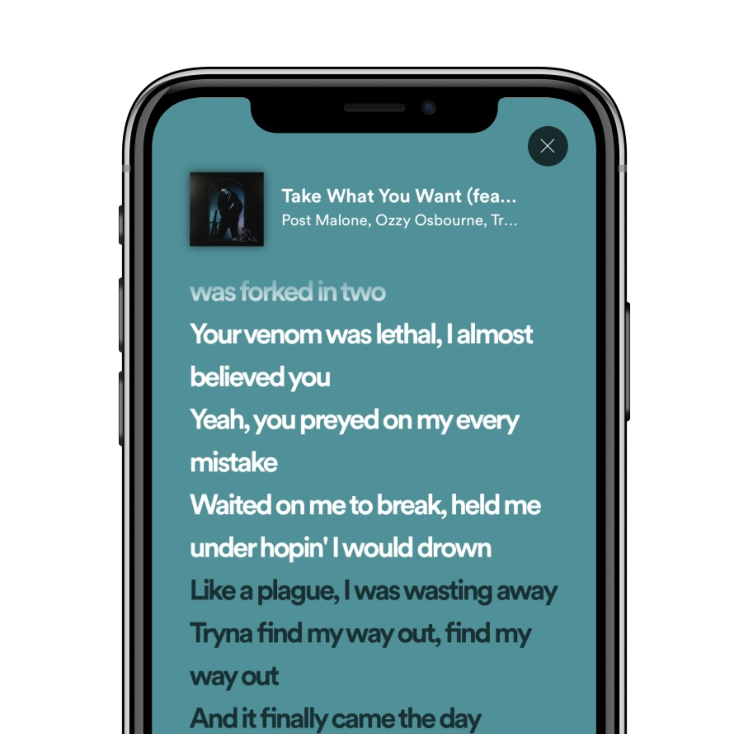
\includegraphics[width=0.4\textwidth]{01-introduction/figures/spotify_lyrics.pdf}
    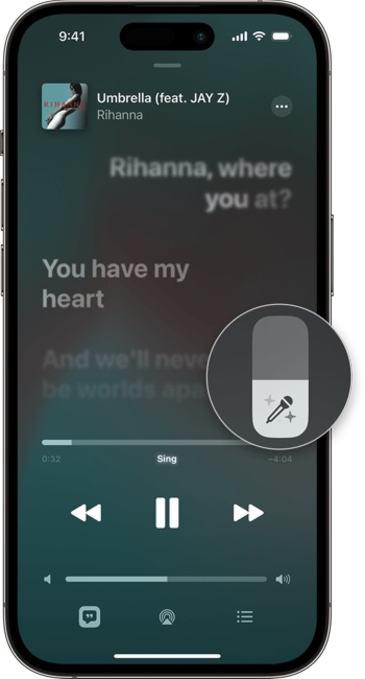
\includegraphics[width=0.2\textwidth]{01-introduction/figures/applemusic_lyrics.pdf}
    \caption{Lyrics within Audio Streaming Applications - Spotify and Apple Music}%
    \label{fig:setup0}
\end{figure}

With the advances in the space of deep learning, cloud computing and improved compute and storage prowess, we are today at the cusp of being able to generate machine transcribed song lyrics. The commercial space is lacking good products that can transcribe songs, with all the commercial entities still using expert or human transcription. Similarly, latest advances in the space of Automatic Speech Recognition (ASR) with the advent of Open AI's Whisper model and Meta's Wav2Vec2.0 models, Acoustic Models such as Hidden Markov Model (HMM) and Music Information Retrieval (MIR) growing as a field for identifying singer, instruments etc. make it an interesting problem to solve. Additionally, considering the long tail of songs without any available lyrics, high cost of obtaining lyrics and the lack of consistent quality amongst available lyrics, there is a great deal of interest in being able to provide high quality, machine transcribed song lyrics.

While the problem statement is interesting, solving the problem of transcribing songs to lyrics is an extremely difficult problem to solve \cite{gu2022mm} . The reason is that in addition to all the challenges faced by speech recognition, there is also an additional presence of noise in the form of accompanied instruments or through the stretching or contraction of words by the singer to convey emotions or mood of the song. As a result, current benchmarks in this nascent space of song lyrics transcription have poor evaluation scores when compared with pure speech.

The aim of this thesis is to come up with an improved Songs Lyrics Transcription solution that can be done by leveraging  state of the art techniques across the domains of Automated Speech Recognition (ASR), Audio Signal Processing and Music Information Retrieval (MIR).

\section{Introduction}
\label{sec:introduction}

Song lyrics transcription is a relatively new field with very little research done in this domain \cite{gao2022automatic}. This domain can be viewed as a co-mingling of three different domains that have overlapping research and application. The three domains include Music Information Retrieval (MIR), Automatic Speech Recognition (ASR) and Acoustic Modelling (AM). In Automatic Speech Recognition (ASR), the core problem is in the speech domain and the goal is to be able to transcribe spoken speech into the text associated with the speech. A more technical definition is given by Jurafsky \cite{jurafsky2000speech} , where he defines ASR as the building of a system for mapping acoustic signals to a string of words \cite{jurafsky2000speech} . Some of the challenges in Automatic Speech Recognition (ASR)  \cite{forsberg2003speech} are that it cannot read body language, which is a significant part of communication for humans, differing accents and pronunciations, difference in spoken and written language etc. Automatic Speech Recognition (ASR) has potential applications in the space of dictation, transcription, voice assistants, searching audio files for particular words etc. Acoustic modelling (AM) establishes statistical representations for features generated from audio speech signals\cite{karpagavalli2016review}. Through acoustic modelling techniques such as using Hidden Markov Models (HMM), Automatic Speech Recognition (ASR) has been performed by leveraging decoding techniques based on decoding concatenated text or phonemes. Hidden Markov Models (HMM) are the engine behind modern Automatic Speech Recognition (ASR) systems and while deep learning models have brought significant improvements to the acoustic modelling part, the Automatic Speech Recognition (ASR) systems themselves have not changed much \cite{gales2008application}. Music Information Retrieval (MIR) is the domain that is historically concerned with the extraction and inference of meaningful features from music (audio signal), symbolic representations of music, indexation of music for retrieval or recommendation purposes.


\begin{figure}[H]
    \centering
    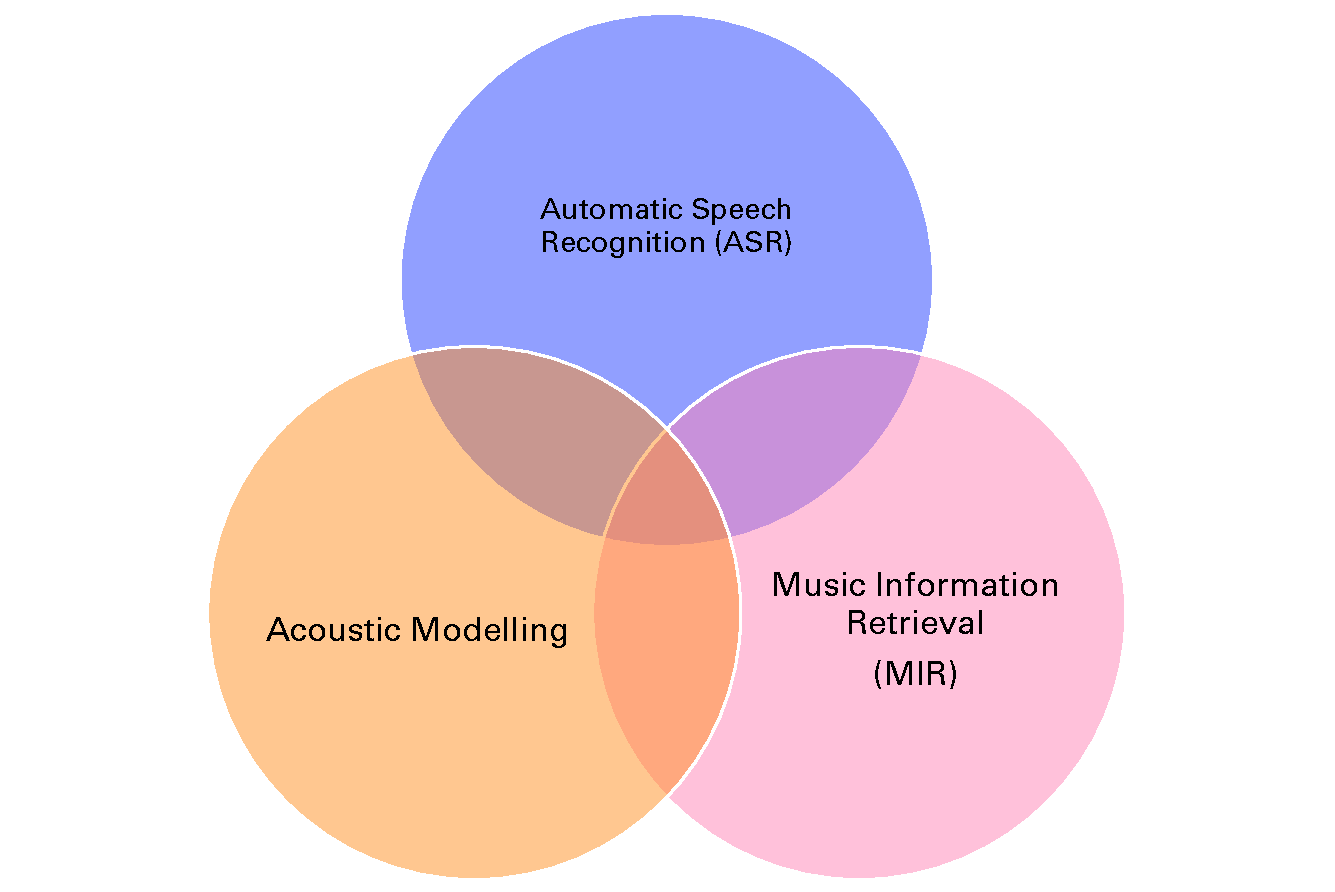
\includegraphics[width=\textwidth]{01-introduction/figures/between_three_domains.pdf}
    \caption{Song Lyrics Transcription as an intersection of multiple domains}%
    \label{fig:setup1}
\end{figure}

To understand the beginnings, Automatic Speech Recognition (ASR) models started in the 1970s in Carnegie Mellon and IBM who introduced the use of discrete density Hidden Markov Models (HMM) and then later at Bell Labs where continuous density Hidden Markov Models (HMM) were introduced. Initially, discrete word speaker dependent large vocabulary models or whole word small vocabulary speaker independent applications were the capability in this field. However, in the early 90s, with the artificial 1000 word Resource Management task, the capability for continuous speaker-independent recognition was built. Post that, through a series of Defense Advanced Research Projects Agency(DARPA) and National Security Agency(NSA) programmes, multilingual transcription of broadcast news programmes and telephone conversations was made possible \cite{gales2008application}. Traditionally, acoustic models have been developed that read the audio signals as spectrograms, specifically in the form of Mel Frequency Cepstral Coefficients, to represent audio signals in spectrogram format.

In our approach, we will be looking at newer deep learning methodologies that have been taking over acoustic models for speech recognition. Through the thesis, we aim to apply this to the songs domain. In our problem statement, we will be interested in exploring techniques in the space of Music Information Retrieval (MIR) to represent songs as spectrograms, understand the way to extract singing voice from the music, termed as Singing voice Separation (SVS), and understanding ways to model music for the Songs Lyrics Transcription task that we will look into.Additionally, we will be specifically interested in the space of fine-tuning self-supervised models such as Wav2vec2.0 that is a recently successful model in the speech domain that leverages unlabelled data to learn representations of audio. Self-supervised learning is a promising technique that we will see in detail in Chapter 2 that limits the necessity of having labeled data for training supervised models. This is particularly useful as unlabelled data in the form of audio is widely available but doing the necessary transcription with the help of humans is an expensive process \cite{baevski2020wav2vec}. We are also interested in the encoder-decoder architecture that is employed in models such as Whisper from Open AI that leverage weakly labelled data \cite{radford2023robust}. We will cover the theoretical foundations in more detail when we come to Chapter 2.

\section{Purpose and Research Question}%
\label{sec:purpose}

In this thesis, the state of the art deep learning architectures will be used to model songs in order to transcribe lyrics in an automatic fashion. We will also propose an evaluation methodologies on the task of songs lyrics transcription. As part of our research study, we will be answering four major questions :

\begin{itemize}
    \item \textbf{Develop Benchmarks in low data scenarios} Can we set up benchmarks for the songs to lyrics transcription problem as there are relatively less data available in this field?
    \item \textbf{Data Augmentation techniques} Does data transformation techniques such as Music Source Separation improve songs to lyrics transcription ?
    \item \textbf{Domain Adaptation Improvement:} Can encoder-side improvements such as transfer learning and decoder-side improvements such as language models improve current benchmarks for songs to lyrics transcription?
    \item \textbf{Encoder-Decoder architectures:} Can pre-trained encoder-decoder architectures improve the current benchmarks for songs to lyrics transcription?

\end{itemize}

\section{Approach and Methodology}

This work focuses on the algorithms and procedures to transcribe songs into lyrics. It focuses on deep learning methods and architectures and the approach to evaluate the problem statement. The approach is to perform literature review into the state of the art techniques in the space of Music Information Retrieval (MIR), Automatic Speech Recognition (ASR) and Acoustic Modelling or Language Modelling techniques (AM/LM) to create an end to end song to lyrics transcription model. As part of the study, we will be iterate through experiments on different architectures, techniques and hyper-parameter tuning to answer the research question and optimize the results. In order to evaluate the research question, we will identify existing metrics or develop a representative metric to understand the quality of transcripts for the song lyrics. The dataset used for the master thesis will be the DALI dataset. To give a background, DALI dataset is the largest corpus of  synchronised Audio, Lyrics and vocal notes \cite{meseguer2020creating}. The dataset will be split and used for training as well as evaluation purposes. To conclude, the process and results will be critically reviewed and compared to one another. Finally, future developments and improvements will be outlined for this topic to be taken further.
